\section*{Appendix}

\section{\LB Event Types}
\label{a:events}
Complete list of all events' names together with their description follows.
% see events.tex.T
\input{events}

\newpage
\section{\LB Job States}
\label{a:jobstat}
Complete list of all job' states together with their description follows.
% see status.tex.T
\input{status}

\begin{figure}[hb]
\centering
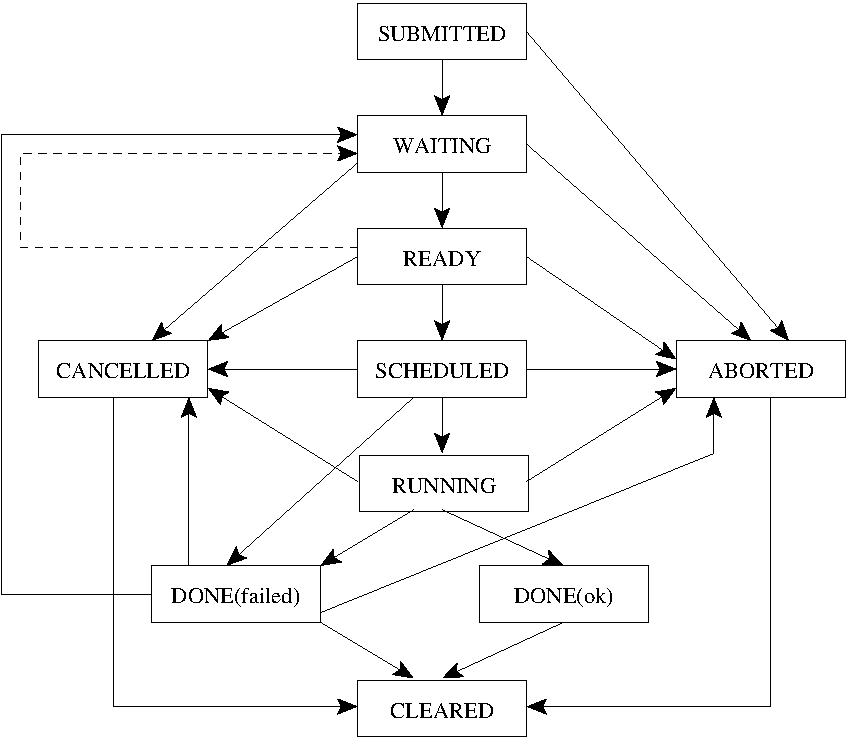
\includegraphics[width=.6\hsize]{images/wms2-jobstat}
\caption{\LB\ job state diagram}
\end{figure}

\newpage
\section{Environment variables}
\label{a:environment}

Complete list of all environment variables affecting LB behaviour follows with 
their description and default values (if applicable).

% default values can be read especially from org.glite.lb.common/src/param.c
% and apropriate header files

\begin{tabularx}{\textwidth}{lX}
GLITE\_WMS\_LOG\_DESTINATION & 
   % see also glite/lb/log_proto.h (org.glite.lb.common/interface/log_proto.h)
   address of \verb'glite-lb-logd' daemon (for logging events), 
   in form \verb'hostname:port',
   default value is \verb'localhost:9002'\\
GLITE\_WMS\_LOG\_TIMEOUT & 
   % see also glite/lb/timeouts.h (org.glite.lb.common/interface/timeouts.h)
   timeout (in seconds) for asynchronous logging, 
   default value is \verb'120' seconds, 
   maximum value is \verb'300' seconds \\
GLITE\_WMS\_LOG\_SYNC\_TIMEOUT & 
   % see also glite/lb/timeouts.h (org.glite.lb.common/interface/timeouts.h)
   timeout (in seconds) for synchronous logging, 
   default value is \verb'120' seconds, 
   maximum value is \verb'600' seconds \\
GLITE\_WMS\_NOTIF\_SERVER & 
   address of \verb'glite-lb-bkserver' daemon (for receiving notifications)
   in form \verb'hostname:port', for receiving notifications,
   there is no default value,
   mandatory for \verb'glite-lb-notify' \\
GLITE\_WMS\_NOTIF\_TIMEOUT & 
   % see also glite/lb/timeouts.h (org.glite.lb.common/interface/timeouts.h)
   timeout (in seconds) for notification registration,
   default value is \verb'120' seconds,
   maximum value is \verb'1800' seconds \\
GLITE\_WMS\_QUERY\_SERVER & 
   address of \verb'glite-lb-bkserver' daemon (for queries), 
   in form \verb'hostname:port', 
   there is no default value \\
GLITE\_WMS\_QUERY\_TIMEOUT &
   % see also glite/lb/timeouts.h (org.glite.lb.common/interface/timeouts.h)
   timeout (in seconds) for queries,
   default value is \verb'120' seconds,
   maximum value is \verb'1800' seconds \\
GLITE\_WMS\_LBPROXY\_STORE\_SOCK &
   UNIX socket location for logging to LB Proxy,
   default value is \verb'/tmp/lb_proxy_store.sock' \\
GLITE\_WMS\_LBPROXY\_SERVE\_SOCK &
   UNIX socket location for queries to LB Proxy,
   default value is \verb'/tmp/lb_proxy_serve.sock' \\
GLITE\_WMS\_LBPROXY\_USER &
   user credentials (DN) when communicating with LB Proxy,  
   there is no default value \\
X509\_USER\_CERT and X509\_USER\_KEY & 
   location of user credentials,
   default values are \verb'~/.globus/usercert.pem' and \verb'~/.globus/userkey.pem' \\
GLOBUS\_HOSTNAME & 
   hostname to appear as event origin, useful only for debugging, 
   default value is hostname \\
QUERY\_SERVER\_OVERRIDE & 
   values defined in QUERY\_SERVER will override also values in jobid in queries,
   useful for debugging only, 
   default value \verb'no' \\
QUERY\_JOBS\_LIMIT & 
   maximal size of results for query on jobs, 
   default value is  \verb'0' (unlimited) \\
QUERY\_EVENTS\_LIMIT & 
   maximal size of results for query on events, 
   default value is  \verb'0' (unlimited) \\
QUERY\_RESULTS & 
   specifies behavior of query functions when size limit is reached,
   value can be \verb'None' (no results are returned),
   \verb'All' (all results are returned, even if over specified limit),
   \verb'Limited' (size of results is limited to size specified by QUERY\_JOBS\_LIMIT
   or QUERY\_EVENTS\_LIMIT) \\
CONNPOOL\_SIZE & 
   maximal number of open connections in logging library,
   for developers only,
   default value is \verb'50' \\
\end{tabularx}

For backward compatibility, all \verb'GLITE_WMS_*' variables can be prefixed by
\verb'EDG_WL_' instead, for example \verb'EDG_WL_LOG_DESTINATION'.
